\begin{figure}
	\centering
	\pgfplotsset{every axis legend/.append style={
		at={(1.05,0.5)},
		anchor=west}}
	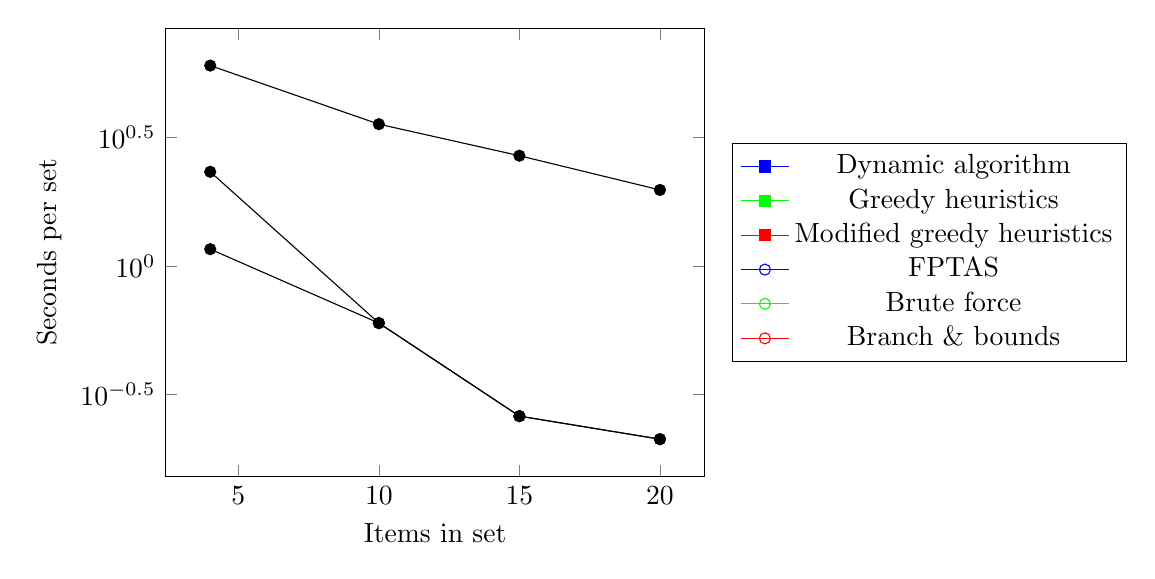
\begin{tikzpicture}
		\begin{semilogyaxis}[
			xlabel=Items in set,
			ylabel=Seconds per set,
			scatter/classes={
				solvePriceDynamic={mark=square*,blue},
				solveHungry={mark=square*,green},
				solveSingle={mark=square*,red},
				fptas={mark=o,blue},
				solveStupid={mark=o,green},
				solveSmart={mark=o,red}
				}
            ]
            
\addplot[scatter,scatter src=explicit symbolic]table[meta=label] {
x y label
4 1.164382 hungryStupidDeviation
10 .600226 hungryStupidDeviation
15 .260588 hungryStupidDeviation
20 .211928 hungryStupidDeviation
};
\addplot[scatter,scatter src=explicit symbolic]table[meta=label] {
x y label
4 2.329300 singleDeviation
10 .600226 singleDeviation
15 .260588 singleDeviation
20 .211928 singleDeviation
};
\addplot[scatter,scatter src=explicit symbolic]table[meta=label] {
x y label
4 6.036380 fptasDeviation
10 3.570200 fptasDeviation
15 2.690720 fptasDeviation
20 1.979910 fptasDeviation
};

			\addlegendentry{Dynamic algorithm}
			\addlegendentry{Greedy heuristics}
			\addlegendentry{Modified greedy heuristics}
			\addlegendentry{FPTAS}
			\addlegendentry{Brute force}
			\addlegendentry{Branch \& bounds}
		\end{semilogyaxis}
	\end{tikzpicture}
\caption{Average time per set with predominant light elements}
\label{plot:lightTime}
\end{figure}
